\documentclass[conference]{IEEEtran}
\usepackage{graphicx}
\usepackage{booktabs}
\usepackage{amsmath}
\usepackage{cite}

\begin{document}

\title{Radar-Led, Camera-Assisted BEV-Language Model for Driving Scene Understanding on nuScenes}

\author{
\IEEEauthorblockN{Aamir Aziz Butt\textsuperscript{1,2}}
\IEEEauthorblockA{\textsuperscript{1}PhD Scholar, Muslim Youth University, Islamabad, Pakistan \\
\textsuperscript{2}Lecturer, Women University of AJ\&K, Bagh, Pakistan \\
amir.butt12@gmail.com}
}

\maketitle

\begin{abstract}
Radar-camera fusion is well established for 3D object detection, but its value for \emph{language-interfaced}
driving-scene understanding -- a model that answers questions about a scene rather than only drawing boxes --
remains largely untested, and existing driving question-answering benchmarks are built on camera and LiDAR alone.
This work trains a small language model (Qwen2.5-0.5B, LoRA-adapted) to answer motion- and speed-related
questions about nuScenes driving scenes from radar point clouds, camera features, and explicit per-object motion
tokens, and evaluates radar's specific, measurable contribution using a majority-answer baseline, a wrong-frame
control that distinguishes genuine sensor use from superficial pattern-matching, and a day/night/rain condition
split. Under oracle (ground-truth) object boxes, radar's contribution is found to be specific rather than diffuse:
every radar-containing model clears the majority baseline on pedestrian-motion counting, while camera alone does
not, and every model's reliance on correct sensor content roughly doubles at night. Replacing oracle boxes with
the project's own trained detector's real predictions, however, collapses the pedestrian-counting result while
leaving car-motion and speed results intact. Seven independently implemented fixes targeting this gap --
class-balanced object-token allocation, detection-threshold tuning, a confidence-score token feature, extended
detector retraining with a full precision/recall sweep, attention-based pillar feature aggregation, auxiliary
LiDAR-occupancy supervision, and cross-modal feature-and-response distillation from a LiDAR teacher detector
nearly $3.3\times$ better on pedestrians -- all fail to recover it, evidence consistent with a sensor-level
limitation of sparse automotive radar for low-radar-cross-section pedestrian targets rather than a fixable
architectural defect.
\end{abstract}

\section{Introduction}
Automotive radar is established as a useful complement to camera for 3D object detection, where the two
modalities' complementary strengths -- camera's semantic richness and radar's direct velocity measurement and
lighting-invariance -- have been repeatedly shown to improve detection accuracy. Whether the same benefit
transfers to a \emph{language}-interfaced driving model -- one that must answer natural-language questions about a
scene, rather than only output bounding boxes -- is comparatively untested: existing driving question-answering
benchmarks are built exclusively on camera and LiDAR, with no radar baseline. This work asks a deliberately narrow
question: can radar measurably improve a language model's ability to answer questions about a driving scene, and
if so, specifically where, and does that improvement survive contact with the project's own, realistically
imperfect object detector rather than only idealized ground truth? Section~\ref{sec:related} positions this
question against existing radar-camera detection work, camera/LiDAR-only driving question-answering benchmarks,
and the handful of contemporary radar-language systems closest to this one. Sections~\ref{sec:method}
and~\ref{sec:results} then present the method and the resulting evidence, including an honest negative result for
one of the two central findings once ground-truth boxes are replaced with real detections.

\section{Related Work}
\label{sec:related}

\subsection{Radar-Camera Fusion for Detection}
Radar-camera fusion is well established for 3D object detection. CenterFusion~\cite{nabati2021centerfusion}
associates radar returns with camera-detected object centers via a frustum-based matching step, using the
associated radar data to improve a camera-only detector's depth, rotation, and velocity estimates, reporting
over a 12\% improvement in nuScenes Detection Score over its camera-only baseline. RCBEVDet~\cite{lin2024rcbevdet}
is a more recent bird's-eye-view fusion approach for the same task. Both confirm that radar-camera fusion is
worth doing for detection; this work's question is whether the same kind of benefit transfers to \emph{language},
a model answering questions rather than drawing boxes. The pillar-based radar encoding used here follows the
general pillarization approach introduced for LiDAR by PointPillars~\cite{lang2019pointpillars}, and the
CenterNet-style heatmap-plus-regression detection head follows the center-based formulation popularized for 3D
detection by CenterPoint~\cite{yin2021centerpoint}.

\subsection{Driving Question-Answering Benchmarks}
NuScenes-QA~\cite{qian2024nuscenesqa}, the benchmark this work's evaluation protocol is built on, is constructed
and baselined entirely on camera and LiDAR detections; radar is not part of its baselines. DriveLM
\cite{sima2024drivelm} is a broader, graph-structured driving question-answering benchmark spanning perception,
prediction, and planning questions, again built on camera and LiDAR with no radar. Neither benchmark tests
whether a camera/LiDAR-centric approach degrades in the conditions -- night, rain -- where radar's physical
advantages (direct velocity measurement, illumination independence) should matter most; Section~\ref{sec:results}-C
directly addresses this gap.

\subsection{Radar-Only and Radar-Language Models}
Two recent systems attempt something closer to a radar-language model. Radar4D-VLM~\cite{han2026radar4dvlm}
reasons over ten consecutive 4D-radar sweeps with no camera input at all, projecting object, scene, and kinematic
tokens into several frozen language-model backbones; it reports that aligned language supervision gave no stable
gain over its direct prediction heads. RLM~\cite{mishra2025rlm} is trained contrastively on over 800,000
radar-caption pairs generated entirely in the CARLA simulator, rather than from real recorded sensor data, and
produces free-form scene similarity rather than the exact-match, ground-truth-checked accuracy used here. Neither
system combines real automotive radar with camera in the radar-led, camera-assisted framing this work uses, and
neither reports a wrong-frame-style control to verify genuine sensor use.

\subsection{Radar-Camera Scene Description and Robust Fusion}
Two contemporaneous systems are closer in spirit. CRaFT-SD~\cite{rangaraj2026craftsd} is a sequential two-stage
vision-language model: a LoRA-fine-tuned VLM reads a rendered range-azimuth map (converted to a pseudo-RGB image)
and writes a structured text description of target position and clutter, which then conditions a second,
pretrained VLM that also sees the camera image to produce a free-text operational-design-domain scene
description. It is evaluated with BLEU score and target range/azimuth regression error (which it reports as
substantially worse than a dedicated detector, 1.7\,m vs.\ 0.11\,m mean range error), rather than exact-match
question-answering accuracy, and it carries no velocity or motion information at all -- its radar representation
is a static power map, not a point cloud with Doppler. RFusion4D~\cite{liang2026rfusion4d} addresses a different
problem, robust 3D detection under adverse weather, with a signal-domain denoising module and a
confidence-aware temporal fusion encoder on high-resolution 4D imaging radar; it reports pedestrian AP of only
7.08\% under adverse weather even with far better radar hardware and two orders of magnitude more training data
than used here, independent evidence for the sensor-level pedestrian-detection ceiling this work documents
directly in Section~\ref{sec:results}-D. Table~\ref{tab:related} summarizes how this work's specific combination
of choices differs from each.

\begin{table*}[t]
\centering
\caption{Positioning relative to related work}
\label{tab:related}
\begin{tabular}{lccccc}
\toprule
Work & Radar type & Data source & Camera & Task & Attribution control \\
\midrule
CenterFusion~\cite{nabati2021centerfusion} & sparse & real & yes & detection & -- \\
Radar4D-VLM~\cite{han2026radar4dvlm} & 4D & real & no & question answering & -- \\
RLM~\cite{mishra2025rlm} & sparse & CARLA simulation & no & free-form captioning & -- \\
CRaFT-SD~\cite{rangaraj2026craftsd} & range-azimuth map & real & yes & free-form captioning & -- \\
RFusion4D~\cite{liang2026rfusion4d} & 4D & real & yes & detection & -- \\
\textbf{This work} & sparse & real & yes & question answering & \textbf{wrong-frame control} \\
\bottomrule
\end{tabular}
\end{table*}

This work's specific, deliberate combination -- real nuScenes data rather than simulation, cheap sparse
automotive radar rather than dense 4D radar, radar \emph{and} camera together rather than radar-only, structured
question-answering rather than free-form captioning, and a wrong-frame control methodology designed so that a
model's answer \emph{sounding} plausible cannot be mistaken for the model \emph{actually using} the sensor -- is
not duplicated by any of the above.

\section{Methodology}
\label{sec:method}

\begin{figure*}[t]
\centering
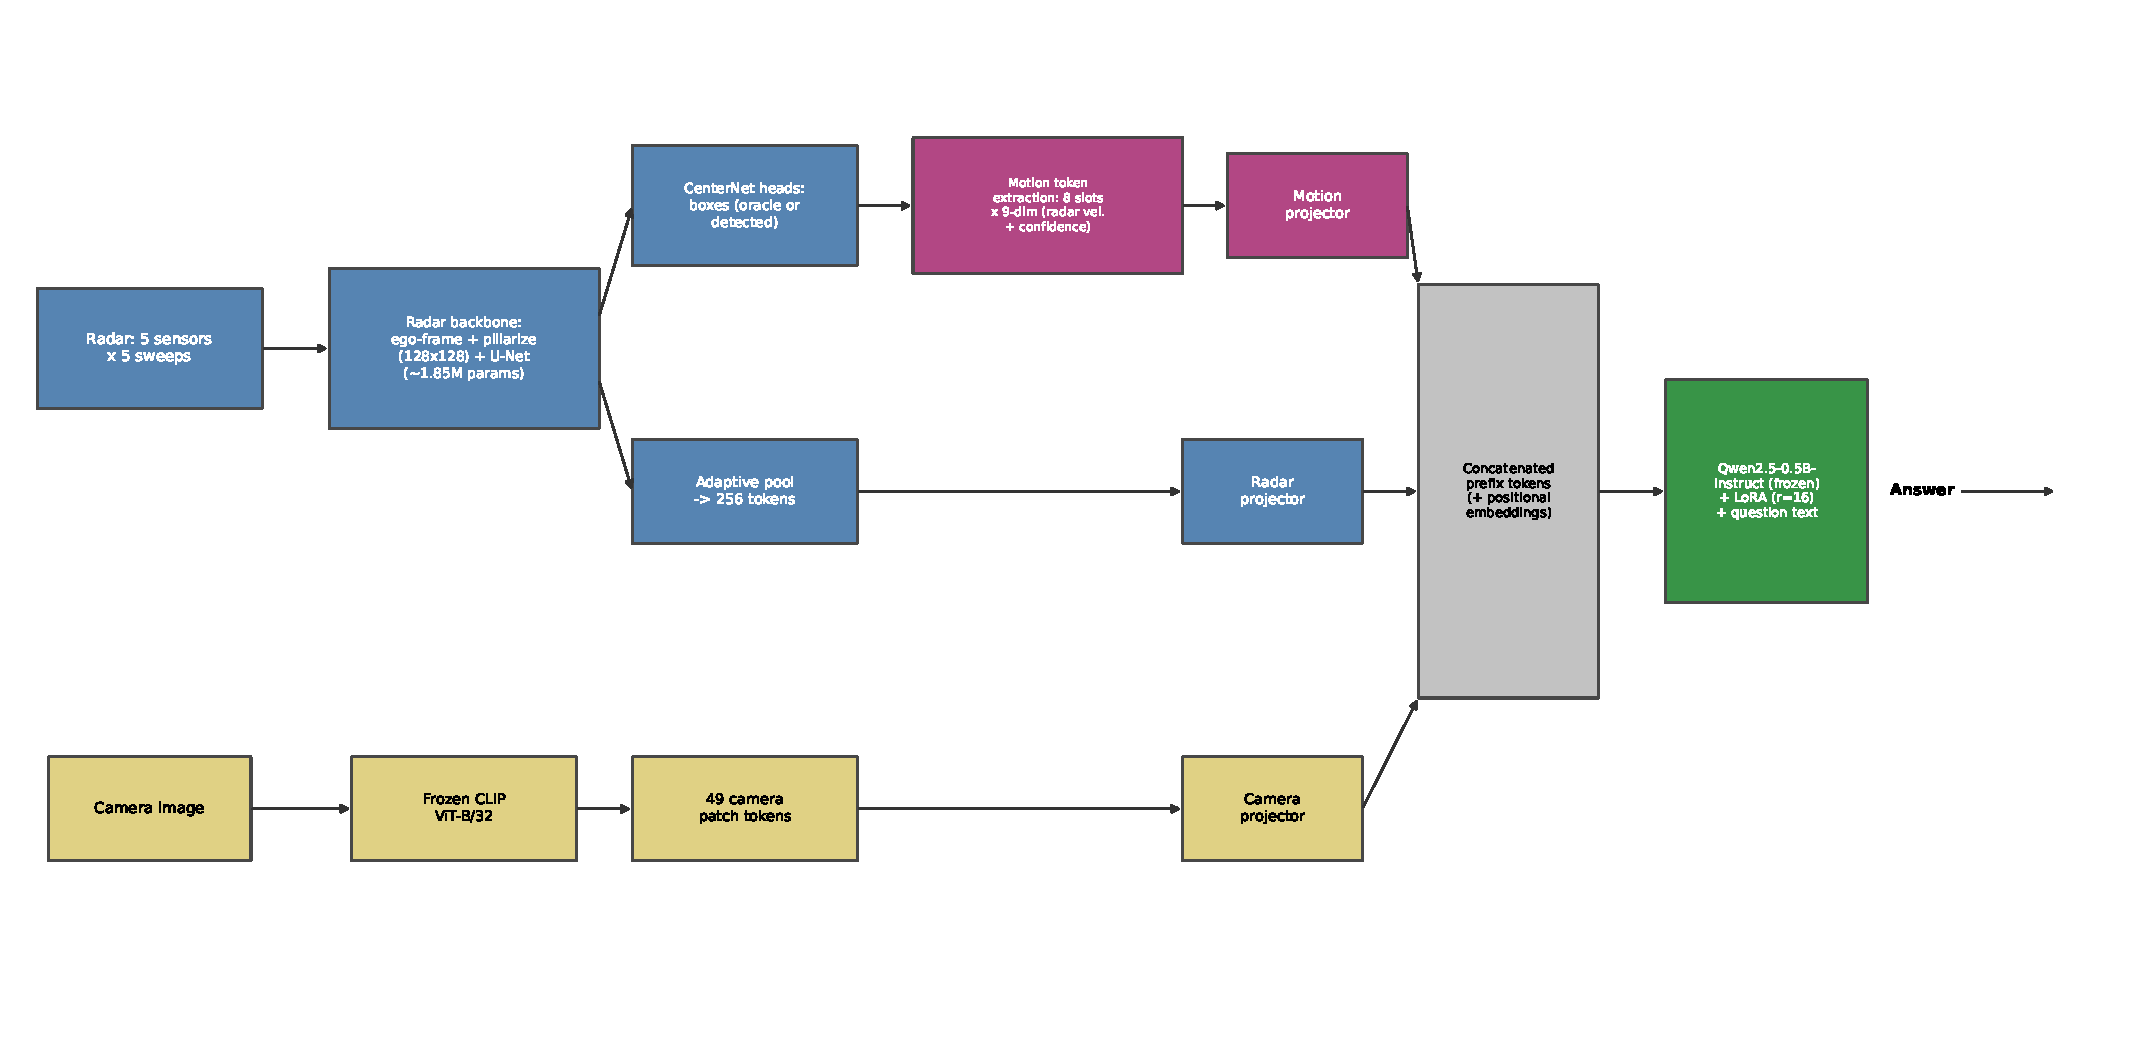
\includegraphics[width=0.92\textwidth]{figures/fig1_architecture.pdf}
\caption{Pipeline overview. Radar sweeps are accumulated in the ego frame, pillarized, and passed through a
shared U-Net backbone that branches into a detection path (CenterNet heads $\to$ boxes $\to$ per-object motion
tokens) and a dense-token path (adaptive pooling to 256 tokens); camera images pass through a frozen CLIP
encoder. Each modality's tokens pass through their own lightweight projector before being concatenated into a
single prefix fed to the LoRA-adapted language model, which generates the answer.}
\label{fig:arch}
\end{figure*}

Fig.~\ref{fig:arch} shows the overall pipeline described in this section.

\subsection{Dataset}
Experiments are conducted on the nuScenes dataset~\cite{caesar2020nuscenes}, using the full v1.0-trainval split:
850 driving scenes (700 for training, 150 for validation), comprising 34{,}149 annotated keyframes collected
across Boston and Singapore under varied weather and lighting conditions, including 84 training scenes tagged
\emph{night} and 138 tagged \emph{rain}. Each keyframe provides six camera images, five radar sensors
(front, front-left, front-right, back-left, back-right), and 3D bounding-box annotations with per-object velocity.
This work restricts attention to the \emph{car} and \emph{pedestrian} categories, and uses the forward-facing
camera as the sole visual input. Fig.~\ref{fig:dataexample} shows a representative keyframe: the front camera
view alongside the corresponding accumulated radar point cloud and ground-truth boxes in the ego-centered BEV
frame used throughout this work.

\begin{figure}[htbp]
\centering
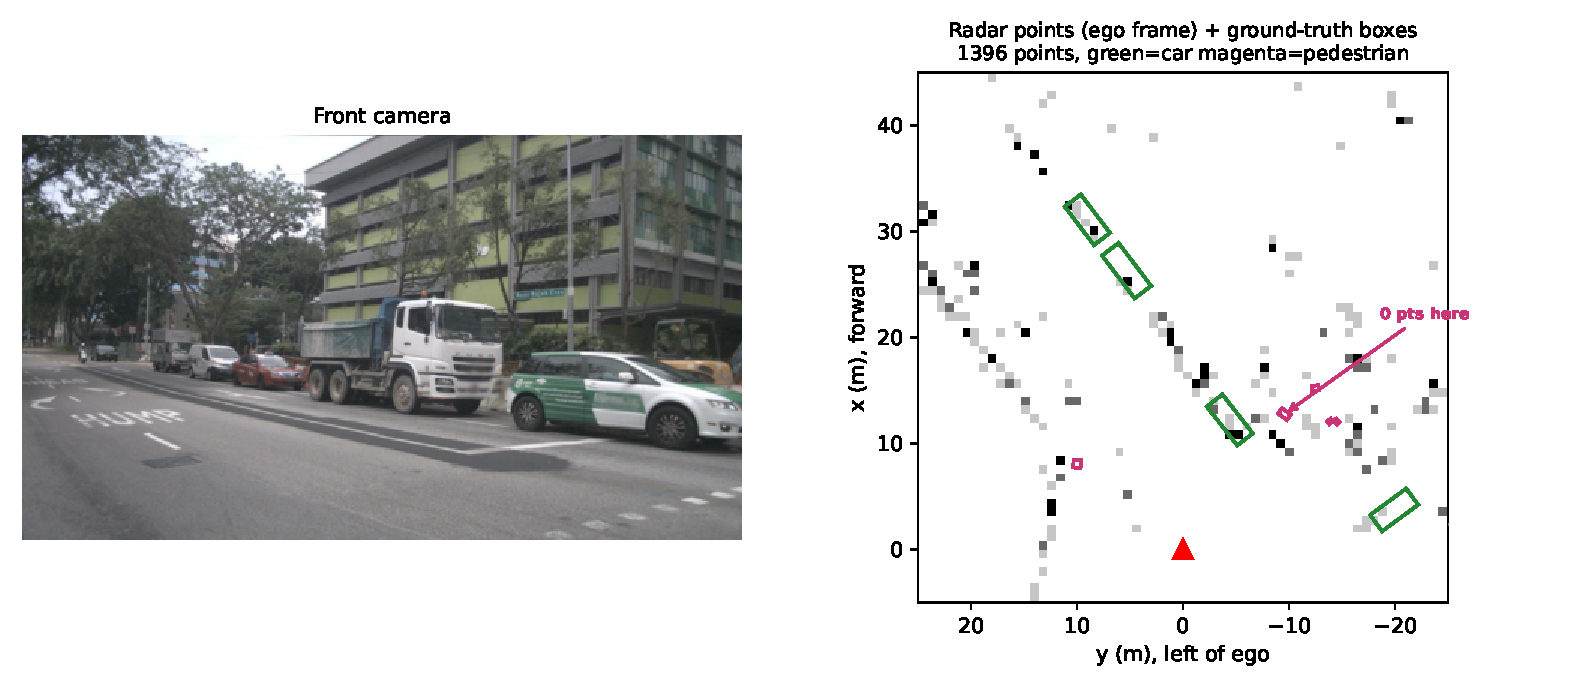
\includegraphics[width=\columnwidth]{figures/fig_data_example.pdf}
\caption{A representative trainval keyframe. Left: front camera. Right: the corresponding 5-sweep-accumulated
radar point cloud (greyscale, darker = more points per BEV cell) with ground-truth boxes overlaid. The
highlighted pedestrian has zero radar points within its box radius, foreshadowing the detection-recall limitation
examined in Section~\ref{sec:results}-D.}
\label{fig:dataexample}
\end{figure}

\subsection{Radar Processing and Detection}
\emph{1) Point Cloud Construction:} Each radar sweep returns a sparse set of reflection points, each with
position $(x,y,z)$, ego-motion-compensated velocity $(v_x,v_y)$, raw radial Doppler velocity $v_r$, and radar
cross-section (RCS). A single sweep yields too few points per object for reliable detection, so the five most
recent sweeps (approx.\ 0.5\,s) from all five radars are accumulated per keyframe, following standard nuScenes
practice. Each point is transformed into the ego vehicle's coordinate frame at keyframe time using the recorded
ego pose and tagged with $dt$, the time elapsed since its own sweep, giving an 8-dimensional feature per point:
$(x,y,z,v_x,v_y,v_r,\text{RCS},dt)$.

\emph{2) Pillarization:} The accumulated point cloud is rasterized onto a $128\times128$ bird's-eye-view grid,
0.8\,m per cell, covering a $102.4\,\text{m}\times102.4\,\text{m}$ window centered on the ego vehicle. Points
falling in the same cell (``pillar'') are summarized by a learned PointNet-style pillar encoder ($\sim$5{,}300
parameters), producing a 64-dimensional feature per occupied pillar and a $128\times128\times64$ bird's-eye-view
tensor per keyframe.

\emph{3) Detector Architecture and Training:} Pillar features pass through a U-Net backbone ($\sim$1.85M
parameters, downsampling then upsampling the spatial grid with skip connections), followed by CenterNet-style
detection heads: a per-class Gaussian heatmap for object centers, plus regression heads for sub-cell offset,
log-size, and sine/cosine heading. Training minimizes a focal loss on the heatmap and an L1 loss on the regression
targets, using AdamW with a one-cycle learning-rate schedule and random left-right mirroring of each training
frame. The detector is trained for 8 epochs on the 700-scene training split; Section~\ref{sec:results}-D reports
that extending this to 20 epochs produces no measurable improvement. At inference, predictions are decoded via
$3\times3$ local-maximum suppression on the heatmap, top-100 selection, and a configurable confidence threshold
(default 0.3).

\emph{4) Detection Performance:} On the 150-scene validation split the detector reaches AP@2m of 0.385 for cars
and 0.120 for pedestrians (Table~\ref{tab:detap}) -- a persistent asymmetry attributable to pedestrians' smaller
radar cross-section and sparser returns, revisited directly in Section~\ref{sec:results}-D.

\subsection{Camera Features}
Camera input is encoded with a frozen, pretrained CLIP ViT-B/32 image encoder~\cite{radford2021clip}, used
strictly as a fixed feature extractor with no fine-tuning. Each image is divided into a $7\times7$ grid of 49
patch tokens (768-dimensional each; the CLS token is discarded), cached per keyframe.

\subsection{Explicit Object (Motion) Tokens}
The dense $128\times128$ pillar grid is adaptively pooled to $16\times16$ (256 tokens) before being passed to the
language model (Section~\ref{sec:method}-E); at this resolution, small or sparse objects such as pedestrians can
be attenuated or lost entirely. To preserve per-object information, an explicit object-token representation is
constructed alongside the dense tokens: up to 8 slots per keyframe, split evenly between the nearest 4 cars and
nearest 4 pedestrians to the ego vehicle, rather than the nearest 8 objects overall -- a shared pool would let the
more numerous car detections crowd pedestrians out of the available slots. Each slot is a 9-dimensional feature
vector:
\[
[\,\text{is\_car},\ \text{is\_ped},\ x,\ y,\ v_x,\ v_y,\ \text{speed},\ \text{has\_pts},\ \text{conf}\,]
\]
where $(x,y)$ is object position (normalized by 50\,m); $(v_x,v_y)$ is not a semantic label but the mean velocity
of radar points falling within a radius of $\max(w,l)/2 + 1.0$\,m of the object center (zero if no points fall
within that radius); \text{has\_pts} is a binary indicator of whether any such points exist; and \text{conf} is
the detector's own classification score for that box, fixed at 1.0 when ground-truth (``oracle'') boxes are used
in place of detector predictions. Empty slots are zero-padded. Two box sources are used across experiments: oracle
(ground-truth annotation) boxes, used to isolate the architectural question of whether object tokens help at all;
and the project's own trained detector's predicted boxes, used in the realistic stress test of
Section~\ref{sec:results}-D.

\subsection{Language Model Architecture and Training}
The backbone language model is Qwen2.5-0.5B-Instruct~\cite{yang2024qwen25}, adapted via Low-Rank Adaptation
(LoRA, rank 16, applied to the query/key/value/output projections of every attention layer, $\alpha=32$, dropout
0.05; 2{,}162{,}688 trainable parameters)~\cite{hu2022lora}, with pretrained weights otherwise frozen. Each sensor
modality is converted into a sequence of soft prompt tokens via its own lightweight projector (LayerNorm
$\to$ Linear $\to$ GELU $\to$ Linear, mapping into the LLM hidden dimension) plus a learned positional embedding
indicating token rank or grid position. The resulting modality-specific token sequences -- 256 radar tokens, 49
camera tokens, and/or 8 object tokens, depending on configuration -- are concatenated and prepended as a prefix
before the question text. In the full-fusion configuration, total trainable parameters (LoRA plus all active
projectors) are 2{,}162{,}688 + 1{,}910{,}416. Training uses AdamW with separate learning rates for the
projector(s) ($10^{-3}$) and LoRA parameters ($2\times10^{-4}$), bf16 mixed precision, batch size 8, for 2 epochs
on a randomly selected subsample of 60{,}000 training questions, evaluated on a disjoint 6{,}000-question
validation subsample.

\subsection{Question Generation}
Two question families are used. NuScenes-QA~\cite{qian2024nuscenesqa} supplies the original benchmark's five
question categories (existence, counting, object identification, status, comparison), templated from
ground-truth scene annotations. To directly probe motion/speed reasoning, three additional question types are
auto-generated from ground-truth object velocities: ``how many cars/pedestrians are moving'' (moving defined as
speed $>0.5$\,m/s) and ``is the fastest moving car's speed slow or fast'' (fast defined as $>8.0$\,m/s; ``none''
if no car is moving). Majority-answer-per-question-type baselines for these three types are 0.195, 0.340, and
0.345 respectively.

\subsection{Evaluation Protocol}
All reported results use exact-match accuracy per question type. Three controls are used throughout:

\emph{Majority-Answer Baseline:} accuracy from always predicting the single most frequent correct answer for a
question type, with no model and no sensor data. Every reported result is interpreted relative to this floor.

\emph{Wrong-Frame Control:} after normal training and evaluation, each model is re-evaluated with sensor tokens
replaced by those of a different, randomly selected keyframe, while question text is unchanged. The resulting
accuracy drop (``wrong-frame gap'') is the primary evidence that a model reads the specific sensor content it was
given, rather than relying on statistical regularities in question wording.

\emph{Condition Split:} every accuracy and wrong-frame-gap figure is additionally computed separately for
keyframes tagged \emph{clear}, \emph{night}, or \emph{rain}, to test whether any sensor's measured advantage
concentrates in the conditions where it has a physical reason to matter.

\section{Results}
\label{sec:results}

\subsection{Detector Performance}
\begin{table}[htbp]
\centering
\caption{Detector AP@2m, full trainval validation split (150 scenes)}
\label{tab:detap}
\begin{tabular}{lc}
\toprule
Class & AP@2m \\
\midrule
Car & 0.385 \\
Pedestrian & 0.120 \\
\bottomrule
\end{tabular}
\end{table}

\subsection{Modality Ablation on Motion/Speed Questions}
All models in Table~\ref{tab:ladder} and Fig.~\ref{fig:ladder} are trained on the identical randomly sampled
60{,}000 training questions and evaluated on the identical 6{,}000-question validation subsample, using oracle
object boxes, isolating the architectural question before addressing detector realism in Section~\ref{sec:results}-D.

\begin{table}[htbp]
\centering
\caption{Motion/speed question accuracy by modality (oracle boxes)}
\label{tab:ladder}
\begin{tabular}{lccc}
\toprule
Model & Overall Acc. & Gap & Peds Moving \\
\midrule
Majority baseline & -- & -- & 0.340 \\
Blind (no sensors) & 0.513 & -- & 0.34 \\
Camera only & 0.544 & +0.053 & 0.33 \\
Radar (dense) only & 0.545 & +0.041 & 0.36 \\
Object tokens only & 0.520 & +0.055 & 0.43 \\
Radar + object tokens & \textbf{0.558} & \textbf{+0.075} & 0.45 \\
Full fusion (+camera) & 0.552 & +0.070 & \textbf{0.47} \\
\bottomrule
\end{tabular}
\end{table}

\begin{figure}[htbp]
\centering
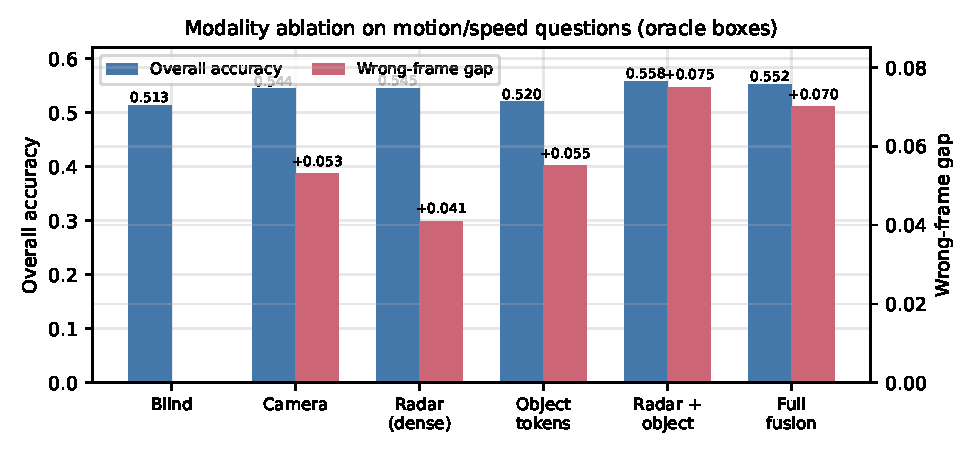
\includegraphics[width=\columnwidth]{figures/fig1_modality_ladder.pdf}
\caption{Overall accuracy and wrong-frame gap across the six modality configurations, oracle boxes.}
\label{fig:ladder}
\end{figure}

\begin{figure}[htbp]
\centering
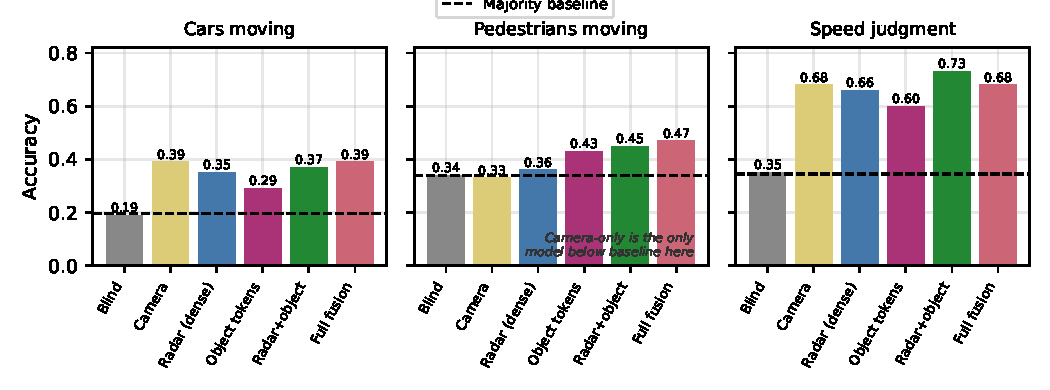
\includegraphics[width=\columnwidth]{figures/fig2_per_question_type.pdf}
\caption{Per-question-type accuracy. Camera alone is the only model that fails to clear the majority baseline
on pedestrian-motion counting; every radar-containing model clears it.}
\label{fig:perq}
\end{figure}

The blind model's near-exact match to the majority baseline on all three question types (Fig.~\ref{fig:perq})
confirms these questions cannot be answered from question-text statistics alone. Camera-only is the only model
that fails to clear the majority baseline on pedestrian-motion counting (0.33 vs.\ 0.34), while every model
containing radar information, in either dense or object-token form, clears it clearly (0.36--0.47). Radar's
measured contribution is therefore not diffuse but specific: it concentrates on pedestrian-motion counting,
consistent with the physical rationale that Doppler velocity is detectable regardless of an object's visual size.
Dense radar features and explicit object tokens are complementary rather than redundant: the dense map's weakest
question type is pedestrian counting, while the object tokens' weakest question types are car counting and
speed; combined, radar + object tokens is the best or joint-best model on every metric, and adding camera on top
yields no further overall improvement.

\subsection{Day/Night/Rain Condition Split}
Fig.~\ref{fig:cond} reports the wrong-frame gap from Table~\ref{tab:ladder}'s models, computed separately for the
4{,}660 clear-condition, 353 night-condition, and 987 rain-condition questions in the validation subsample.

\begin{figure}[htbp]
\centering
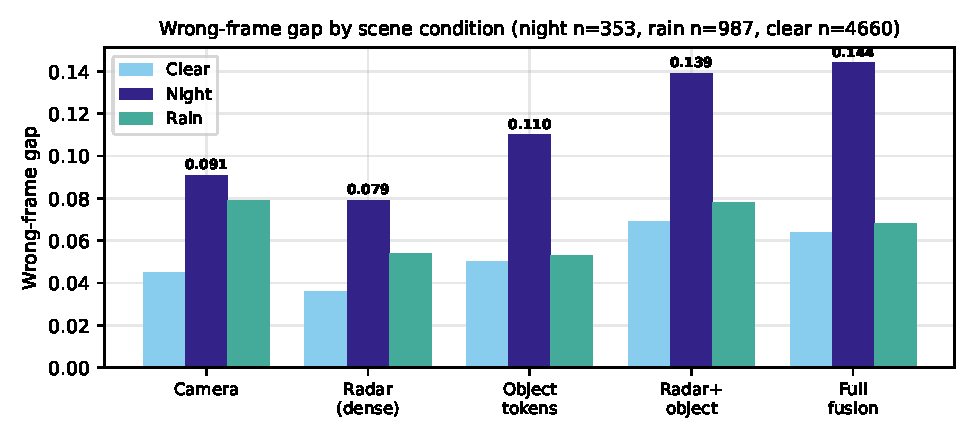
\includegraphics[width=\columnwidth]{figures/fig3_condition_split.pdf}
\caption{Wrong-frame gap by scene condition. Every model's gap roughly doubles at night; the two radar+object
models show the largest night-condition gaps of all.}
\label{fig:cond}
\end{figure}

Every model's wrong-frame gap is larger at night than in clear conditions, roughly doubling in most cases,
indicating that every model relies more heavily on correct sensor content specifically at night. The two
radar-containing object-token models show the largest night-condition gaps, exceeding camera-only's. Given that
night accounts for only 353 of 6{,}000 validation questions, the exact magnitude of each figure carries an
estimated uncertainty of roughly $\pm0.03$; the consistency of direction across five independently trained models
is the more statistically meaningful finding.

\subsection{Real-Detector Stress Test}
Results above use oracle object boxes to isolate the architectural question. Table~\ref{tab:stress} and
Fig.~\ref{fig:stress} repeat the radar + object tokens evaluation with object tokens instead sourced from the
project's own trained detector's predictions, testing whether the pedestrian-counting finding survives realistic,
imperfect detection.

\begin{table}[htbp]
\centering
\caption{Pedestrian-counting accuracy under four independently tested configurations}
\label{tab:stress}
\begin{tabular}{lccc}
\toprule
Configuration & Overall & Gap & Peds Moving \\
\midrule
Oracle boxes & 0.558 & +0.075 & \textbf{0.45} \\
Detected, balanced, 0.3 thr & 0.519 & +0.039 & 0.37 \\
Detected, balanced, 0.15 thr & 0.546 & +0.049 & 0.36 \\
Detected, +confidence, 0.3 thr & 0.541 & +0.048 & 0.36 \\
Detected, +confidence, 0.15 thr & 0.553 & +0.050 & 0.35 \\
\bottomrule
\end{tabular}
\end{table}

\begin{figure}[htbp]
\centering
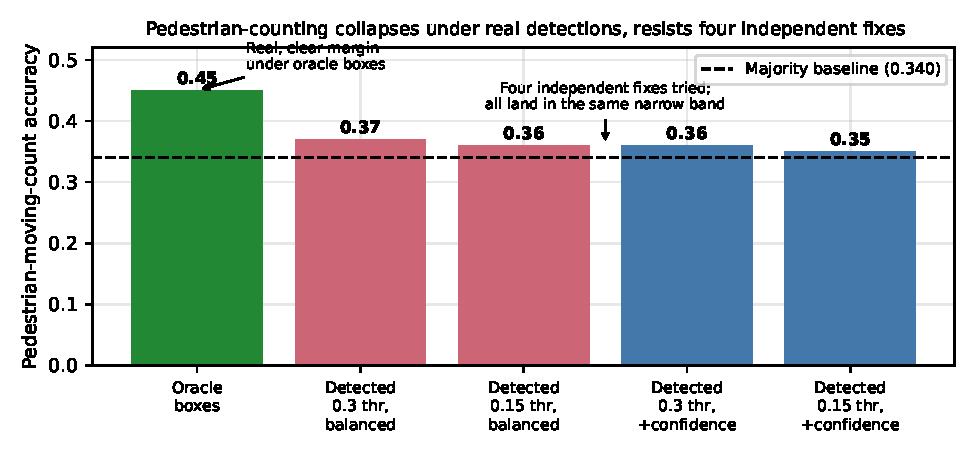
\includegraphics[width=\columnwidth]{figures/fig4_stress_test.pdf}
\caption{Pedestrian-counting accuracy collapses when switching from oracle to detected boxes, and stays collapsed
across four independently tried fixes.}
\label{fig:stress}
\end{figure}

Car-motion counting and speed judgment are robust to the switch from oracle to detected boxes (within
approximately 0.02 of their oracle values across all four detected configurations). Pedestrian-motion counting is
not: it falls from 0.45 to 0.35--0.37 across every detected configuration tested, a drop that persists despite
three independently implemented interventions: (i) class-balanced slot allocation, ruling out cars crowding
pedestrians out of the 8 available slots; (ii) a lower detection confidence threshold (0.15 vs.\ the default
0.3), ruling out pedestrian detection recall as the limiting factor; and (iii) an explicit confidence-score
feature added to each object token, letting the model learn to discount low-confidence detections. None recovers
pedestrian-counting accuracy.

A fourth intervention -- retraining the detector for 20 epochs (2.5$\times$ the original 8) with per-epoch
checkpointing, plus a full precision/recall sweep across seven confidence thresholds (0.05--0.40) on the
retrained checkpoint (Fig.~\ref{fig:pr}) -- was also tested. Both classes' validation AP plateaued by epoch 7--9
and did not improve further (car AP 0.385 $\to$ 0.378; pedestrian AP 0.120 $\to$ 0.109), and no threshold yields a
usable pedestrian operating point (recall does not exceed approximately 0.27, reached only at a precision of
approximately 0.04).

\begin{figure}[htbp]
\centering
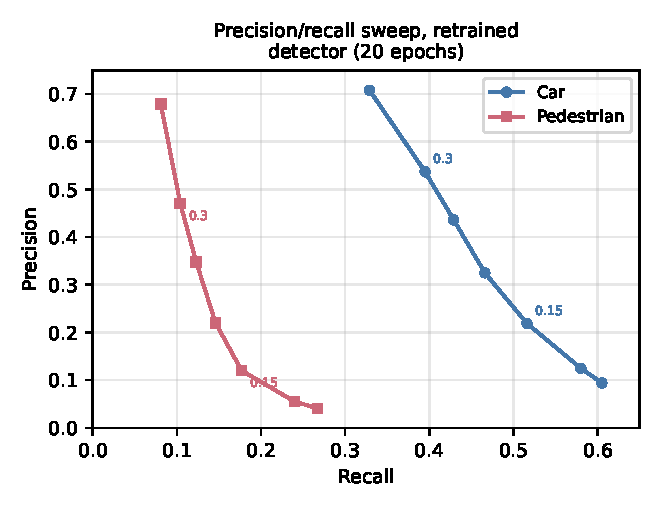
\includegraphics[width=0.85\columnwidth]{figures/fig5_pr_sweep.pdf}
\caption{Precision/recall sweep of the retrained detector. The car curve offers a usable operating range; no
point on the pedestrian curve offers acceptable precision and recall simultaneously.}
\label{fig:pr}
\end{figure}

With four token-level and training-budget interventions exhausted, three further architectural interventions were
tested, each going further than the last toward genuinely richer supervision. \emph{Fifth}, the pillar encoder's
max-pooling aggregation -- which keeps only the single loudest point per channel per pillar, discarding the rest
-- was replaced with learned attention pooling, letting the network combine several points gradedly rather than
keep only one. \emph{Sixth}, an auxiliary training-time-only loss was added: nuScenes' own keyframe LiDAR sweep
was rasterized onto the same BEV grid as a dense occupancy target, and a small head was trained to predict it from
radar features alone, injecting outside information during training while leaving the detector's architecture and
inference-time inputs unchanged. \emph{Seventh}, a full LiDAR-only teacher detector (identical CenterNet-style
architecture, LiDAR points in place of radar points) was trained and confirmed to be substantially stronger than
the radar detector, then distilled into the radar student via feature distillation (cosine distance between
student and frozen-teacher BEV feature maps) and response distillation (BCE between the student's heatmap logits
and the teacher's sigmoid heatmap as a soft target), following CRKD~\cite{song2024crkd}.

\begin{table}[htbp]
\centering
\caption{Detector AP under three further architectural interventions}
\label{tab:detfixes}
\begin{tabular}{lcc}
\toprule
Detector & Car AP@2m & Ped AP@2m \\
\midrule
Original radar (baseline) & 0.385 & 0.120 \\
Attention-pooling (fix 5) & 0.383 & 0.117 \\
LiDAR-aux occupancy (fix 6) & 0.384 & 0.118 \\
LiDAR teacher (reference ceiling) & \textbf{0.720} & \textbf{0.400} \\
Distilled radar, CRKD-style (fix 7) & 0.383 & 0.116 \\
\bottomrule
\end{tabular}
\end{table}

Fig.~\ref{fig:radarvlidar} shows why the teacher is a meaningful reference ceiling rather than a marginal one: in
a representative keyframe, the nearest pedestrian has zero radar points within its box radius (even after
5-sweep accumulation) against 18 LiDAR points in the same radius from a single sweep. Despite this real density
gap and a teacher nearly $3.3\times$ better on pedestrian AP, all three interventions land in the same narrow
band as the first four (Table~\ref{tab:detfixes}) -- statistically indistinguishable from the original detector.
The distillation losses were not inert: feature-distillation loss fell from 0.352 to 0.274 and
response-distillation loss from 0.099 to 0.092 over training, indicating the student genuinely moved toward the
teacher's representations. This did not translate into additional detections. Because detector AP did not change
under any of the three interventions, and every configuration in Table~\ref{tab:stress} shows detector AP change
and downstream pedestrian-counting change moving together, the full downstream language-model re-evaluation was
not repeated for these three detectors.

\begin{figure}[htbp]
\centering
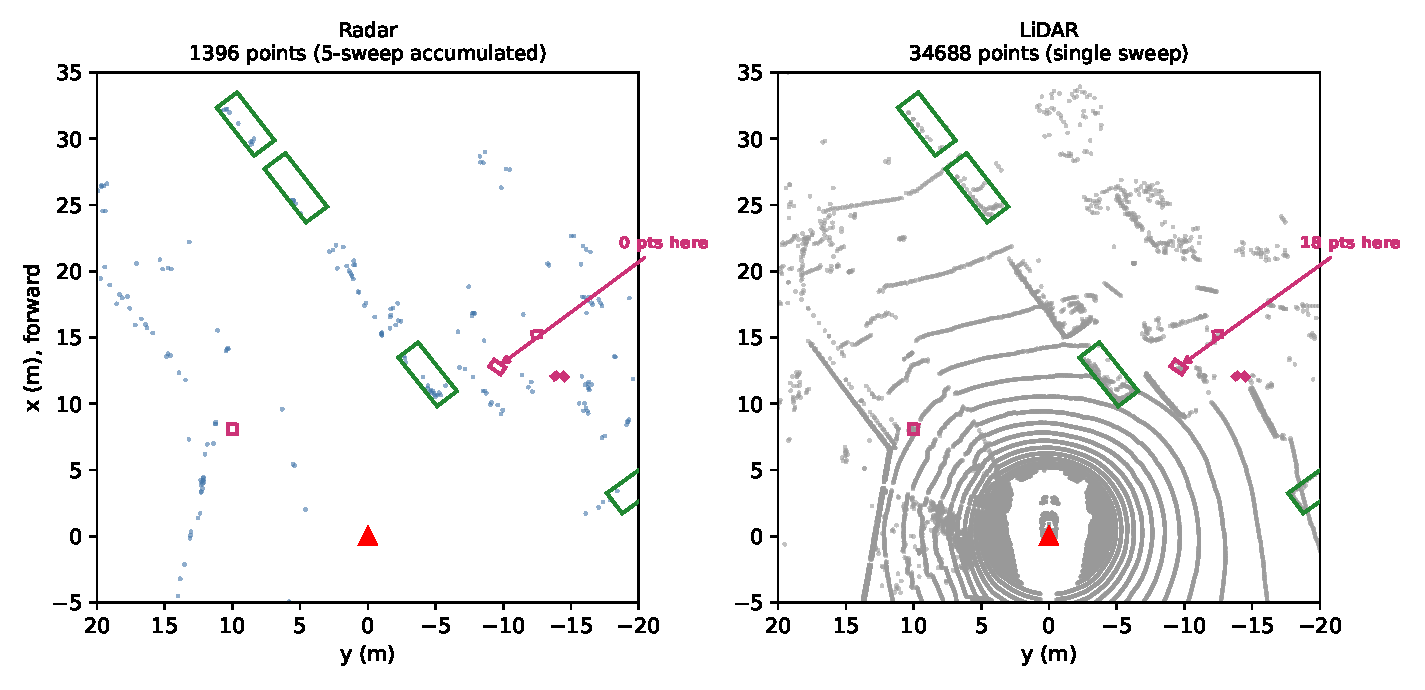
\includegraphics[width=\columnwidth]{figures/fig_radar_vs_lidar.pdf}
\caption{Radar (5-sweep accumulated) vs.\ LiDAR (single sweep) points in the same keyframe. The highlighted
pedestrian has zero radar points within its box radius against 18 LiDAR points in the same radius -- a concrete
case of the absent-information failure mode Table~\ref{tab:detfixes} points to.}
\label{fig:radarvlidar}
\end{figure}

All seven candidate fixes for the pedestrian-counting problem -- spanning token design, detection thresholding,
confidence-awareness, detector training budget, feature aggregation, auxiliary dense supervision, and real
cross-modal distillation from a verified, substantially richer teacher -- have now been tried independently, and
all seven failed to recover it. The seventh is the strongest evidence of all: genuine knowledge transfer from a
sensor that triples pedestrian AP could not move the radar student's own detections. This is consistent with the
limitation living in the radar student's \emph{input} rather than in how that input is processed -- if the sparse
points needed to recognize a pedestrian were never captured, no amount of smarter aggregation, auxiliary
supervision, or distillation pressure can manufacture detections from information that was never there.

\subsection{Summary of Findings}
Seven independently implemented and isolated interventions -- object-token slot allocation, detection threshold,
a confidence-score token feature, extended detector training with a full precision/recall sweep, attention-based
pillar feature aggregation, auxiliary LiDAR-occupancy supervision, and cross-modal feature-and-response
distillation from a verified, substantially richer LiDAR teacher -- each targeting a specific hypothesis for the
pedestrian-counting regression, all failed to close the gap between oracle and detected conditions. This
convergent null result across seven architecturally unrelated interventions, including one that injects genuine
outside information via a teacher nearly $3.3\times$ better on pedestrian AP, is strong evidence against a
fixable pipeline defect and consistent with a sensor-level limitation: pedestrians present a substantially lower
radar cross-section and sparser, less consistent returns than vehicles, a limitation independently observed even
with higher-resolution 4D imaging radar, two orders of magnitude more training data, and dedicated signal-domain
denoising in contemporaneous work~\cite{liang2026rfusion4d} (pedestrian AP of 7.08\% under adverse weather, versus
a 5.47\% camera-only baseline). The results reported here therefore support a claim narrower than ``radar
improves driving-scene question answering broadly'': radar's measured contribution is robust and specific to
car-motion and speed reasoning under both idealized and realistic detection conditions, and additionally robust
for pedestrian-motion reasoning only under idealized (oracle) conditions.

\section{Discussion and Limitations}
The night-condition result (Section~\ref{sec:results}-C) was obtained under oracle boxes only and has not yet
been re-tested under the project's own detector's predictions; this is a direct item for future work, alongside
multi-seed confidence intervals on the headline gaps. The pedestrian-counting ceiling documented in
Section~\ref{sec:results}-D suggests a concrete design implication rather than a dead end: for vulnerable road
users specifically, a camera-led, radar-assisted framing may be more appropriate than the radar-led framing
supported here for vehicles.

\section{Conclusion}
This work presents a controlled, ablation-based evaluation of radar's contribution to a language-interfaced
driving-scene model, using a wrong-frame control and a day/night/rain condition split to separate genuine sensor
use from superficial pattern-matching. Radar's contribution to car-motion counting and speed judgment is shown to
be real and robust to realistic detector noise. Radar's contribution to pedestrian-motion counting is shown to be
real under idealized conditions but is not yet demonstrated under realistic ones, after seven independently tried
and isolated fixes -- including cross-modal distillation from a LiDAR teacher nearly $3.3\times$ better on
pedestrian detection -- a result best explained by a sensor-level limitation of sparse automotive radar for
low-radar-cross-section targets, corroborated by an independent contemporary study.

\begin{thebibliography}{00}
\bibitem{caesar2020nuscenes} H. Caesar et al., ``nuScenes: A multimodal dataset for autonomous driving,'' in
\emph{Proc. CVPR}, 2020.
\bibitem{radford2021clip} A. Radford et al., ``Learning transferable visual models from natural language
supervision,'' in \emph{Proc. ICML}, 2021.
\bibitem{yang2024qwen25} A. Yang et al., ``Qwen2.5 Technical Report,'' \emph{arXiv:2412.15115}, 2024.
\bibitem{hu2022lora} E. J. Hu et al., ``LoRA: Low-rank adaptation of large language models,'' in \emph{Proc.
ICLR}, 2022.
\bibitem{qian2024nuscenesqa} T. Qian et al., ``NuScenes-QA: A multi-modal visual question answering benchmark for
autonomous driving scenario,'' in \emph{Proc. AAAI}, 2024.
\bibitem{liang2026rfusion4d} W. Liang, M. Lei, T. Wang, and B. Cheng, ``Robust fusion of 4-D radar and camera for
all-weather perception in autonomous driving,'' \emph{IEEE Open J. Intell. Transp. Syst.}, vol. 7, 2026.
\bibitem{nabati2021centerfusion} R. Nabati and H. Qi, ``CenterFusion: Center-based radar and camera fusion for 3D
object detection,'' in \emph{Proc. WACV}, 2021, pp. 1527--1536.
\bibitem{lin2024rcbevdet} Z. Lin et al., ``RCBEVDet: Radar-camera fusion in bird's eye view for 3D object
detection,'' in \emph{Proc. CVPR}, Jun. 2024, pp. 14928--14937.
\bibitem{lang2019pointpillars} A. H. Lang, S. Vora, H. Caesar, L. Zhou, J. Yang, and O. Beijbom, ``PointPillars:
Fast encoders for object detection from point clouds,'' in \emph{Proc. CVPR}, 2019.
\bibitem{yin2021centerpoint} T. Yin, X. Zhou, and P. Kr\"ahenb\"uhl, ``Center-based 3D object detection and
tracking,'' in \emph{Proc. CVPR}, Jun. 2021, pp. 11784--11793.
\bibitem{sima2024drivelm} C. Sima et al., ``DriveLM: Driving with graph visual question answering,'' in
\emph{Proc. ECCV}, 2024.
\bibitem{han2026radar4dvlm} J. Han et al., ``Radar4D-VLM: Proposal-grounded temporal 4D radar reasoning across
frozen language models,'' \emph{arXiv:2608.04130}, 2026.
\bibitem{mishra2025rlm} A. Mishra, A. Bansal, and D. Bharadia, ``RLM: A vision-language model approach for radar
scene understanding,'' \emph{arXiv:2511.21105}, 2025.
\bibitem{rangaraj2026craftsd} P. A. Rangaraj, T. Alkanat, and A. Pandharipande, ``Camera--radar data-based vision
language model for automotive driving scene description,'' \emph{IEEE Sensors J.}, vol. 26, no. 13,
pp. 20469--20476, Jul. 2026.
\bibitem{song2024crkd} L. Song, J. Cheng, et al., ``CRKD: Enhanced camera-radar object detection with
cross-modality knowledge distillation,'' in \emph{Proc. CVPR}, 2024.
\end{thebibliography}

\end{document}
